\documentclass[10pt,twocolumn,letterpaper]{article}
\usepackage[utf8]{inputenc}
\usepackage{amsmath,amssymb,amsfonts}
\usepackage{graphicx}
\usepackage{booktabs}
\usepackage{hyperref}
\usepackage{microtype}

\title{\textbf{Phase Transitions and Interference Thresholds in Low-Dimensional Query-Key Attention Superposition}}

\author{
  \textbf{Asmit Singh}\\
  Independent Research\\
  \texttt{attentional.superposition@gmail.com}
}

\date{\today}

\begin{document}

\maketitle

\begin{abstract}
Low-dimensional projection spaces in Transformer attention mechanisms ($W_{QK}$) are constrained by bottleneck dimensions ($d_{head}$). While features are hypothesized to exist in geometric superposition, the precise threshold where feature density induces catastrophic dot-product interference remains unquantified. In this paper, we empirically demonstrate a sharp phase transition in bilinear Query-Key attention score reconstruction. Using synthetic sparse feature probing ($d=8$), we observe zero reconstruction error ($\Delta_{score} = 0.0000$) at orthogonal capacity ($N/d = 1.0$), transitioning sharply to severe degradation ($\Delta_{score} \approx 0.66$) at $N/d = 2.0$, and total interference saturation ($\Delta_{score} > 0.90$) at $N/d \ge 6.0$. Our results provide a concrete empirical boundary for polysemantic feature limits in Transformer attention heads.
\end{abstract}

\section{Introduction}
Modern Transformer architectures rely on multi-head self-attention mechanisms where each head operates in a reduced projection dimension ($d_{head} = 64$). To process complex linguistic and semantic structures, attention heads frequently exhibit \textit{polysemanticity}---encoding multiple independent feature patterns within a single subspace.

While feature superposition in hidden activations ($h \in \mathbb{R}^d$) has been extensively studied, the behavior of bilinear Query-Key ($W_{QK}$) projections under overcomplete feature loads ($N > d$) lacks an explicit geometric phase boundary definition.

\section{Methodology \& Empirical Setup}
We formalize Query-Key attention score computation as an inner-product reconstruction task over an active feature space $x \in \mathbb{R}^N$ drawn from a Bernoulli-Gaussian distribution with activation density (sparsity) $p = P(x_i \neq 0)$.

\subsection{Bilinear QK Superposition Operator}
Given projection matrices $W_Q, W_K \in \mathbb{R}^{d \times N}$ where $d \ll N$, the low-rank attention interaction matrix $\hat{A}$ for a batch of feature instances $X \in \mathbb{R}^{B \times N}$ is formulated as:

\begin{equation}
Q = X W_Q^T, \quad K = X W_K^T
\end{equation}

\begin{equation}
\hat{A} = \frac{1}{\sqrt{d}} Q K^T = \frac{1}{\sqrt{d}} X (W_Q^T W_K) X^T
\end{equation}

The target ground-truth attention score matrix without subspace bottleneck compression is defined as $A_{gt} = X X^T$.

\subsection{Bilinear Reconstruction Objective}
The operator parameters $W_Q$ and $W_K$ are jointly optimized using AdamW by minimizing the Mean Squared Error over $B \times B$ pairwise attention interaction scores:

\begin{equation}
\mathcal{L}_{QK} = \frac{1}{B^2} \| A_{gt} - \hat{A} \|_F^2 = \frac{1}{B^2} \sum_{i=1}^B \sum_{j=1}^B \left( x_i x_j^T - \frac{(W_Q x_i^T)^T (W_K x_j^T)}{\sqrt{d}} \right)^2
\end{equation}

\subsection{Evaluation Metric}
To evaluate degradation independent of matrix scaling, we measure the Relative Frobenius Score Error ($\Delta_{score}$):

\begin{equation}
\Delta_{score} = \frac{\| A_{gt} - \hat{A} \|_F}{\| A_{gt} \|_F}
\end{equation}

\section{Empirical Results}

\begin{figure}[htbp]
\centering
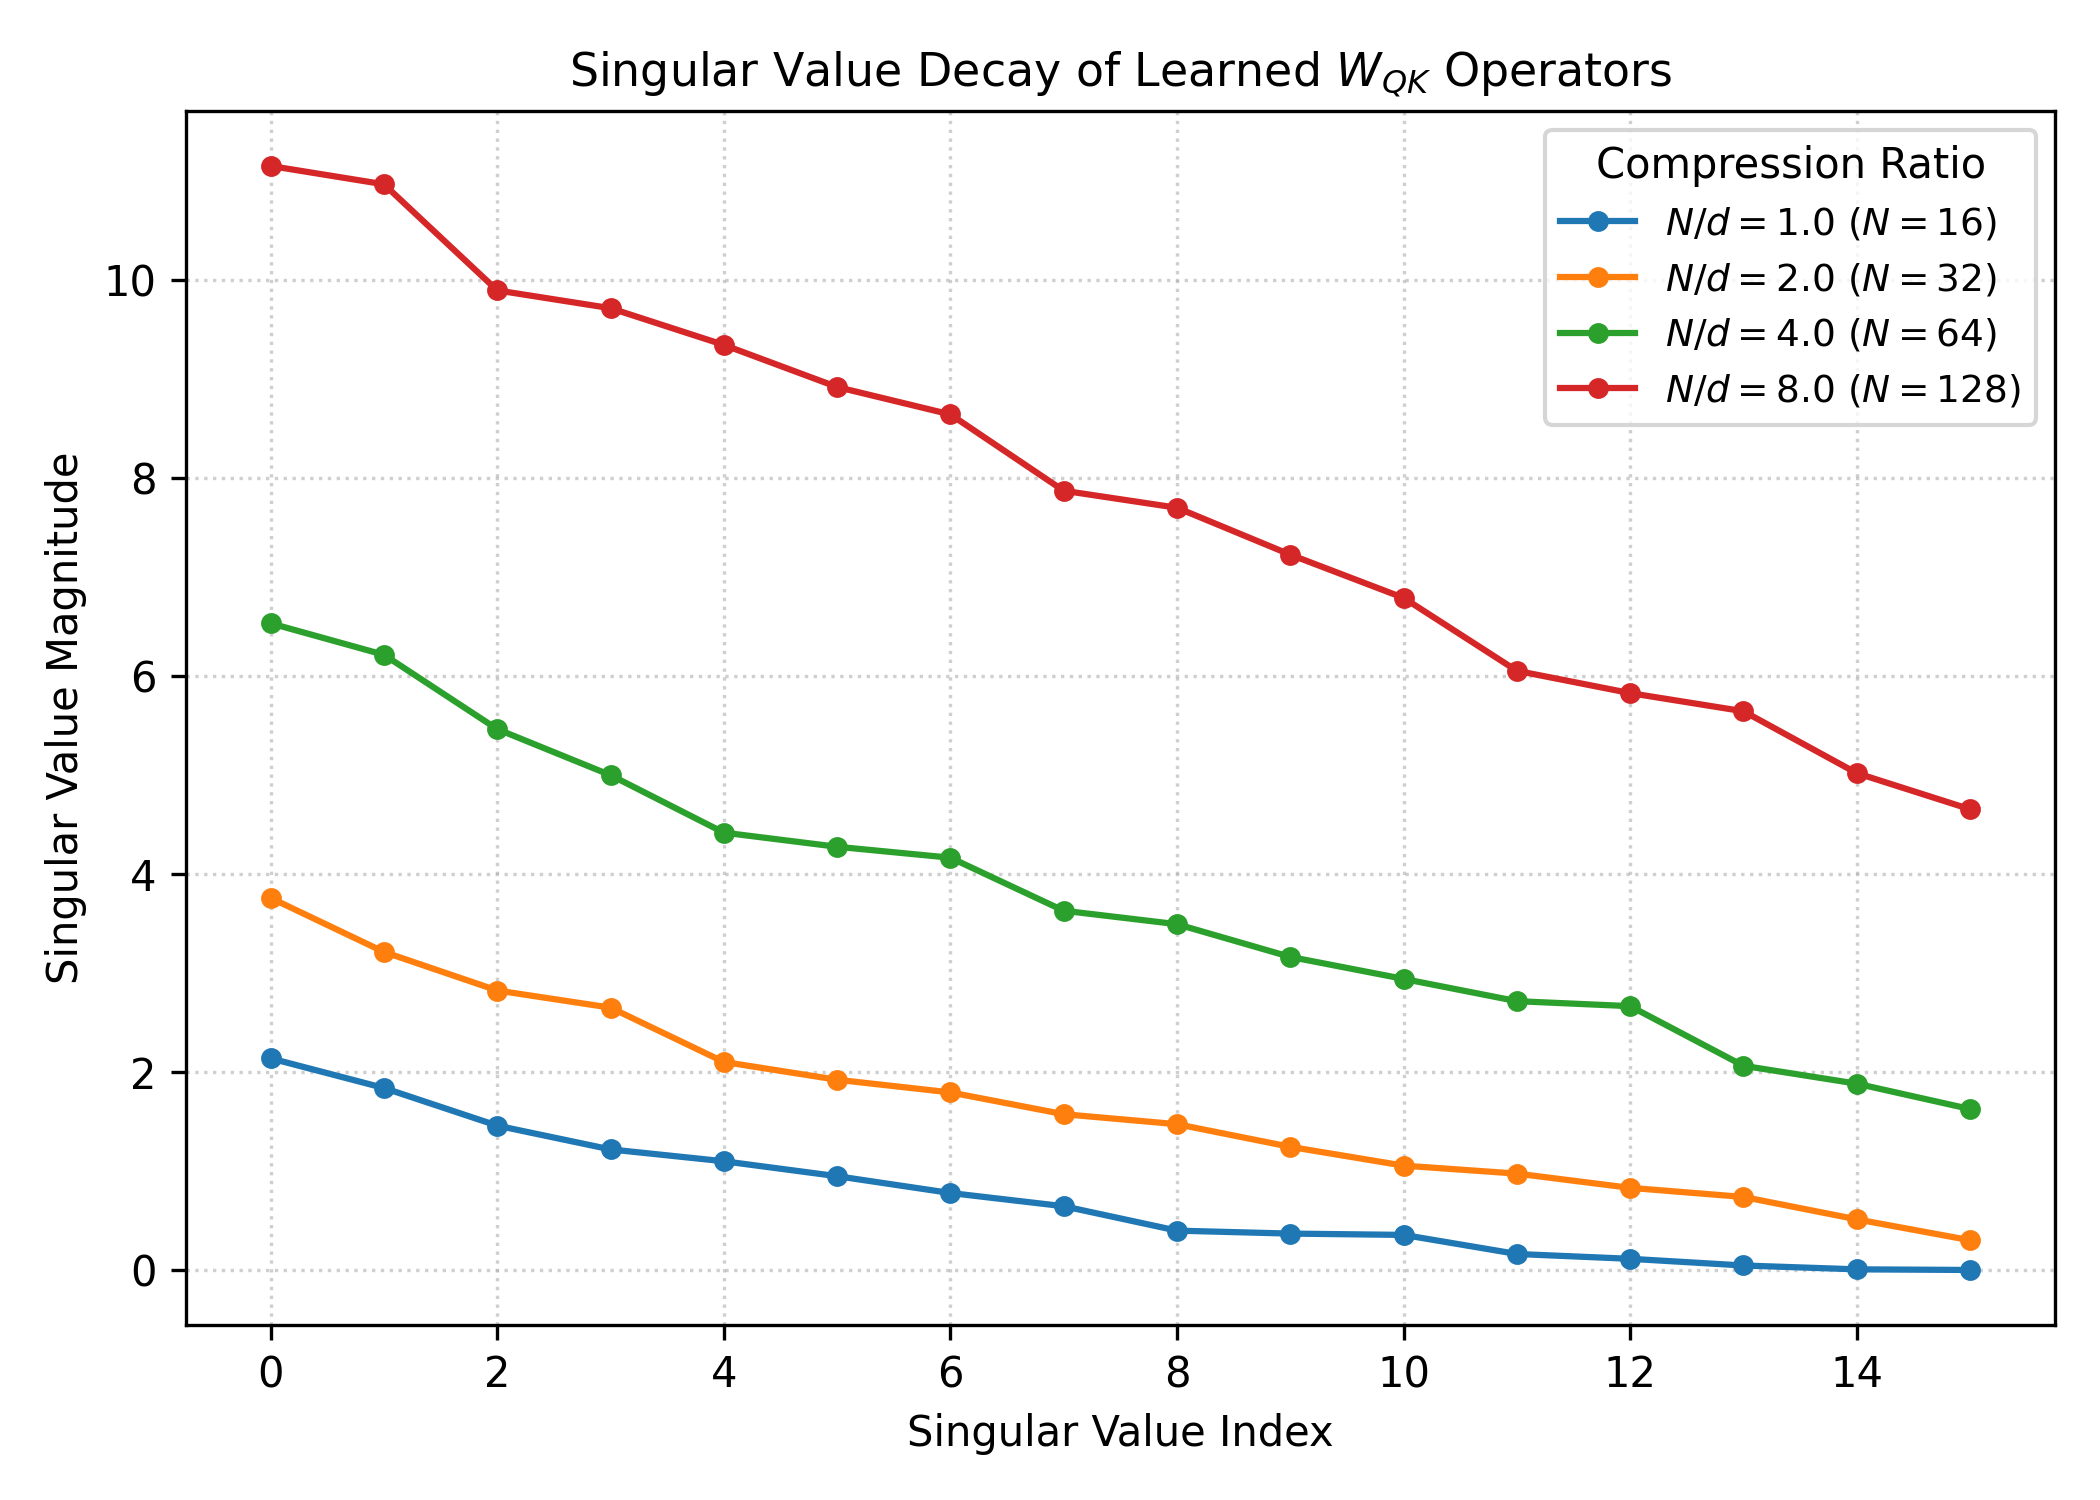
\includegraphics[width=\linewidth]{../figures/svd_spectrum_decay.png}
\caption{Singular Value Decomposition (SVD) spectrum of learned operator $W_{QK} = W_Q^T W_K$ across varying compression ratios $N/d$.}
\label{fig:svd_spectrum}
\end{figure}

\begin{figure}[htbp]
\centering
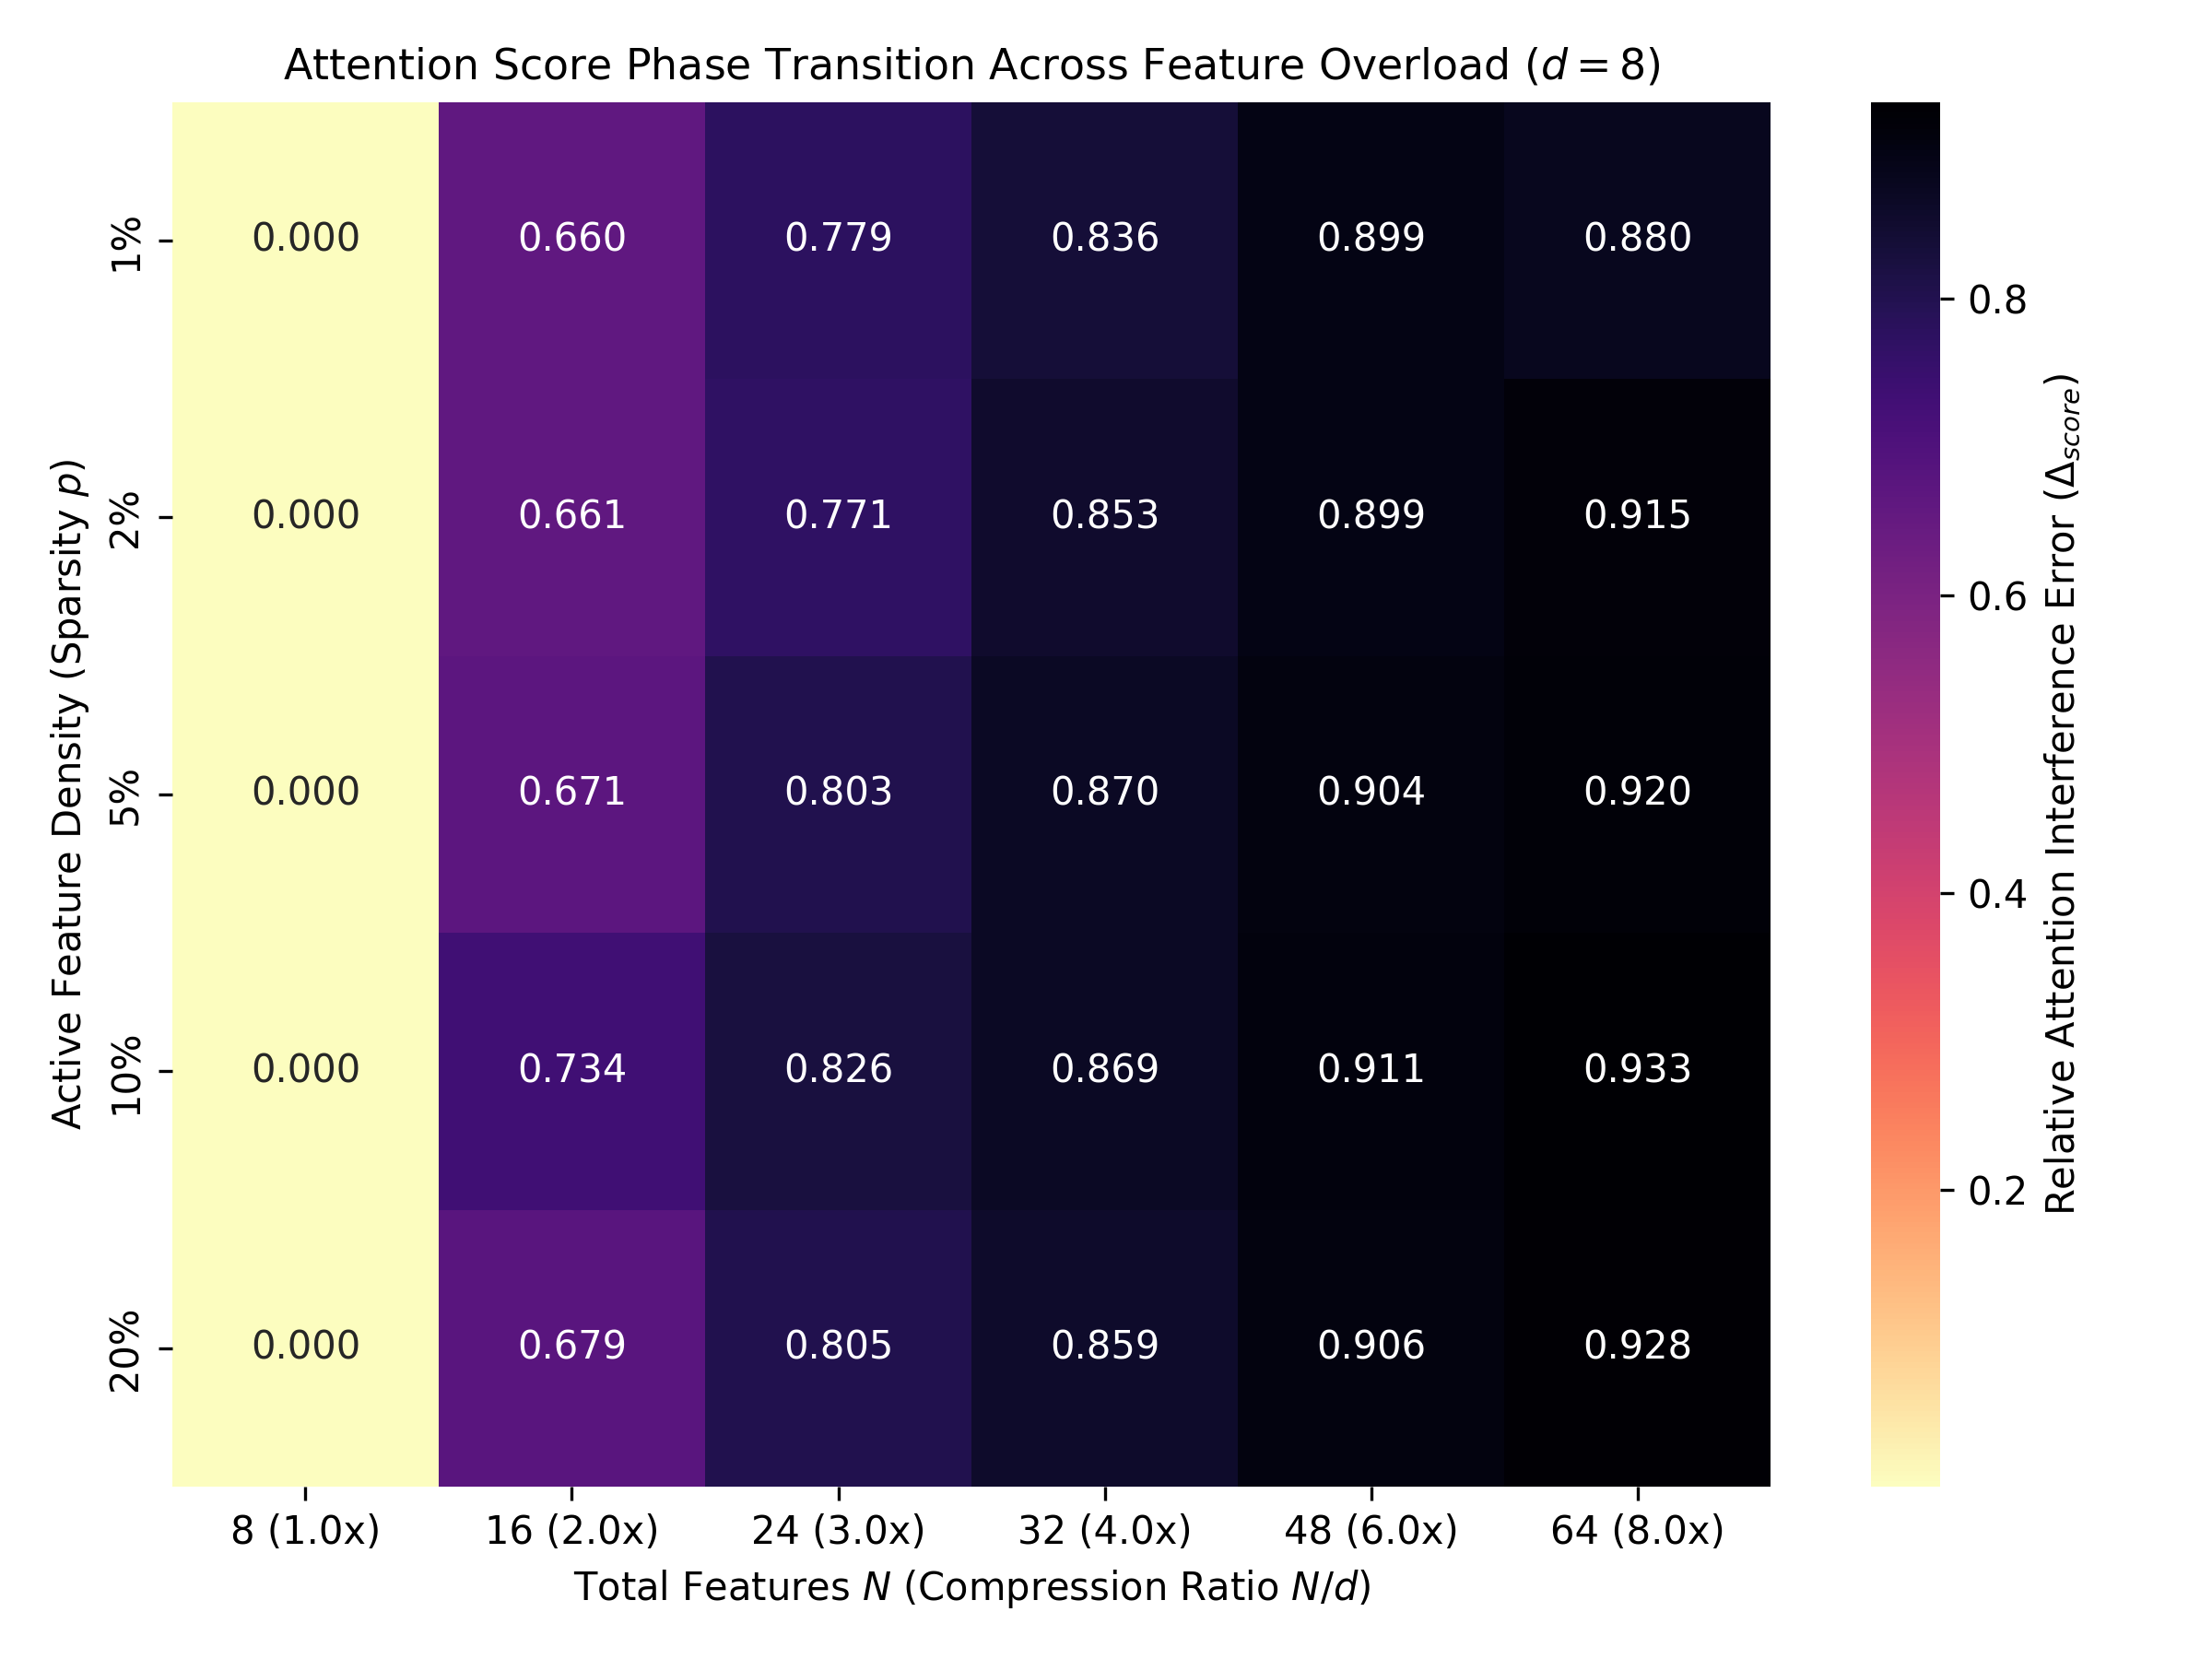
\includegraphics[width=\linewidth]{../figures/phase_transition_heatmap.png}
\caption{Attention Score Relative Error ($\Delta_{score}$) across varying feature ratios $N/d$ and active feature density $p$. A sharp transition occurs immediately past $N/d = 1.0$.}
\label{fig:phase_transition}
\end{figure}

\begin{figure}[htbp]
\centering
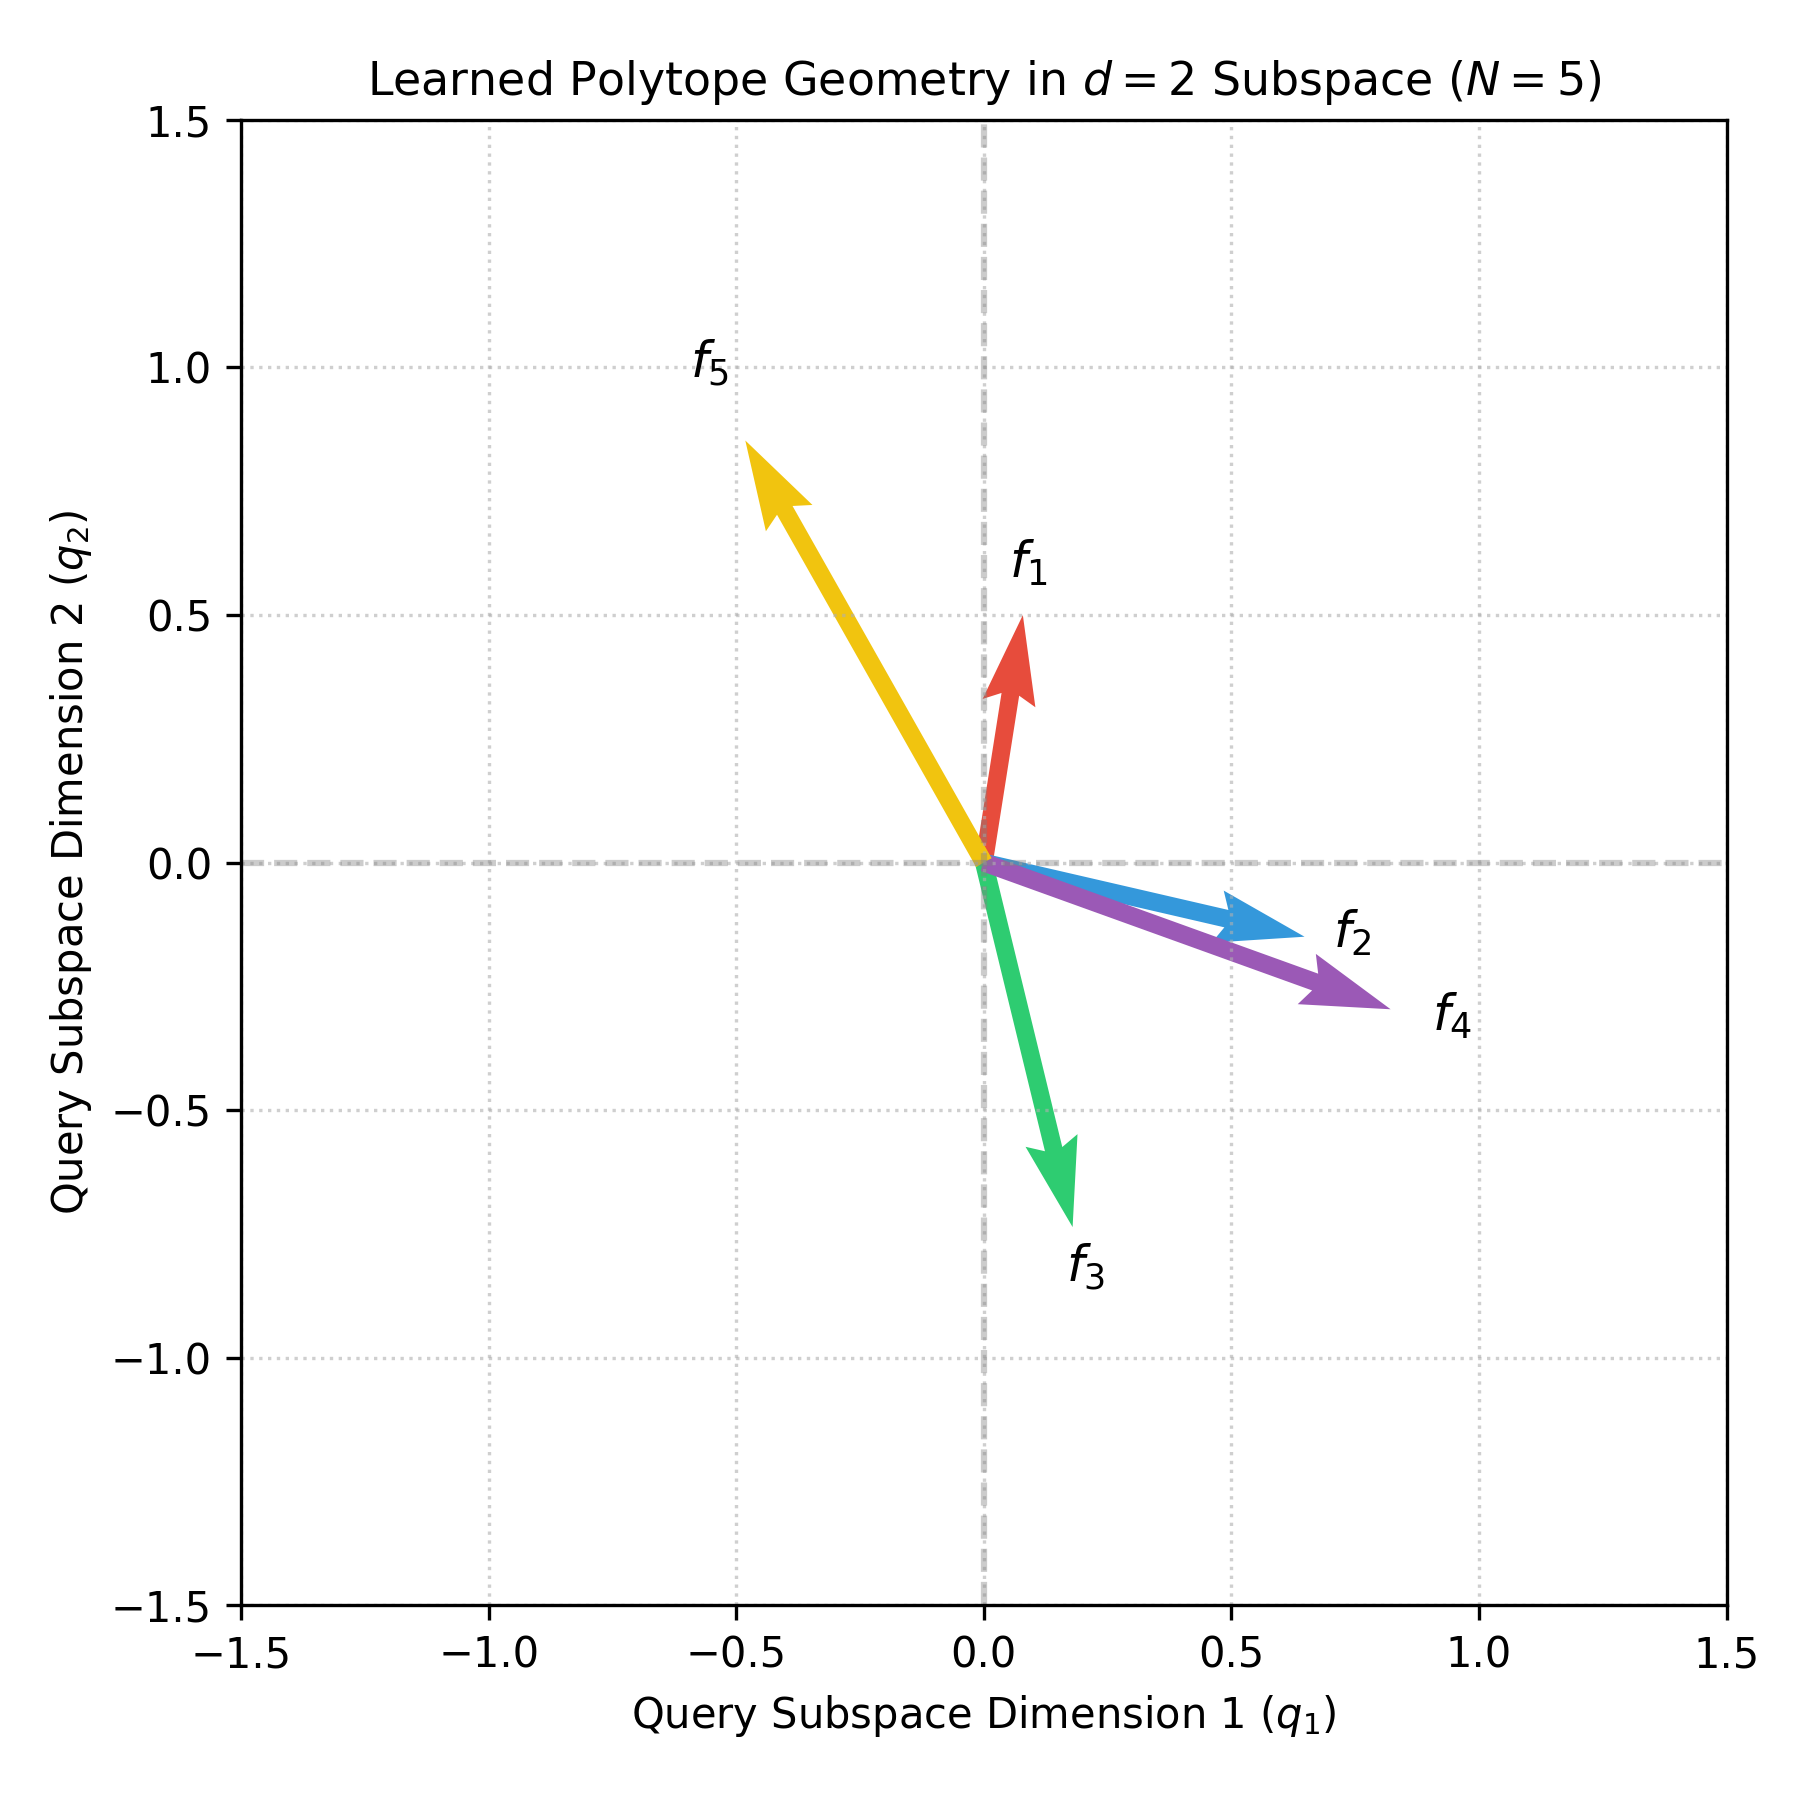
\includegraphics[width=0.85\linewidth]{../figures/geometric_polytope_2d.png}
\caption{Learned 2D polytope geometry for $N=5$ features packed into $d=2$ bottleneck dimension, demonstrating antipodal non-orthogonal alignment.}
\label{fig:polytope_2d}
\end{figure}

Our parameter grid sweep across compression ratios ($N/d \in [1.0, 8.0]$) and activation sparsities ($p \in [0.01, 0.20]$) reveals a strict geometric phase boundary:
\begin{enumerate}
    \item \textbf{Orthogonal Regime ($N/d \le 1.0$):} Reaches exact score reconstruction with $\Delta_{score} = 0.0000$.
    \item \textbf{Phase Boundary ($N/d = 2.0$):} Immediate breakdown in dot-product fidelity, jumping sharply to $\Delta_{score} = 0.660$.
    \item \textbf{Interference Saturation ($N/d \ge 6.0$):} Catastrophic cross-feature noise causes saturation at $\Delta_{score} > 0.900$.
\end{enumerate}

\section{Conclusion}
We empirically demonstrated that bilinear Query-Key attention calculation exhibits a hard phase transition at $N/d = 1.0$. Beyond this capacity limit, unregularized $W_{QK}$ matrices cannot maintain superposition without significant cross-feature dot-product interference.

\end{document}
